%--------------------------------------------------------------------
%--------------------------------------------------------------------
% Formato para los talleres del curso de Herramientas Computacionales
% Universidad de los Andes
%--------------------------------------------------------------------
%--------------------------------------------------------------------

\documentclass[11pt,letterpaper]{exam}
\usepackage[utf8]{inputenc}
\usepackage[spanish]{babel}
\usepackage{graphicx}
\usepackage{mdframed}
\usepackage{tabularx}
\usepackage[absolute]{textpos} % Para poner una imagen completa en la portada
\usepackage{multirow}
\mdfdefinestyle{mystyle}{leftmargin=1cm,rightmargin=1cm,linecolor=red}
%\usepackage{pst-barcode}
%\usepackage{auto-pst-pdf}
\usepackage{xcolor}
\usepackage{hyperref}
\hypersetup{colorlinks=false,linkbordercolor=red,linkcolor=green,pdfborderstyle={/S/U/W 1}}
\decimalpoint


\newcommand{\base}[1]{\underline{\hspace{#1}}}
\boxedpoints
\pointname{ pt}
%\extrawidth{0.75in}
%\extrafootheight{-0.5in}
\extraheadheight{-0.15in}
%\pagestyle{head}

%\noprintanswers
%\printanswers
\renewcommand{\solutiontitle}{}
\SolutionEmphasis{\color{blue}}

\usepackage{upquote,textcomp}
\newcommand\upquote[1]{\textquotesingle#1\textquotesingle} % To fix straight quotes in verbatim

\begin{document}
\begin{center}
{\Large Herramientas Computacionales} \\
Taller 6 - \textsc{Python - Matplotlib} \\
{\small \it marzo de 2015}
\end{center}

\begin{textblock*}{40mm}(10mm,20mm)
  
\includegraphics[width=3cm]{logoUniandes.pdf}
\end{textblock*}

\begin{textblock*}{40mm}(161mm,20mm)
  
\includegraphics[width=3cm]{logoUniandes.pdf}
\end{textblock*}

\vspace{1cm}

La solución de este taller debe ser presentada en un solo archivo comprimido con nombre \verb+NombreApellido_HW6.zip,+ en el cual estén contenidas las respuestas a los dos ejercicios, bien sea en scripts, bien sea en notebooks de iPython. Tiene dos semanas para resolverlo y vale por dos.

\begin{questions}

\question[20] {\bf{Impresora radical}} 
\begin{parts}
\part[10] Escriba código en Python que de como resultado un \verb+array+ con los enteros entre 1 y 25 impresos en zigzag como muestra la figura. Es obligatorio usar arrays de \verb+numPy+.
\part[10] Luego utilice \verb+imshow+ para producir la figura mostrada a la derecha, use la opción \\ \verb+interpolation='None'+.

\begin{center}
	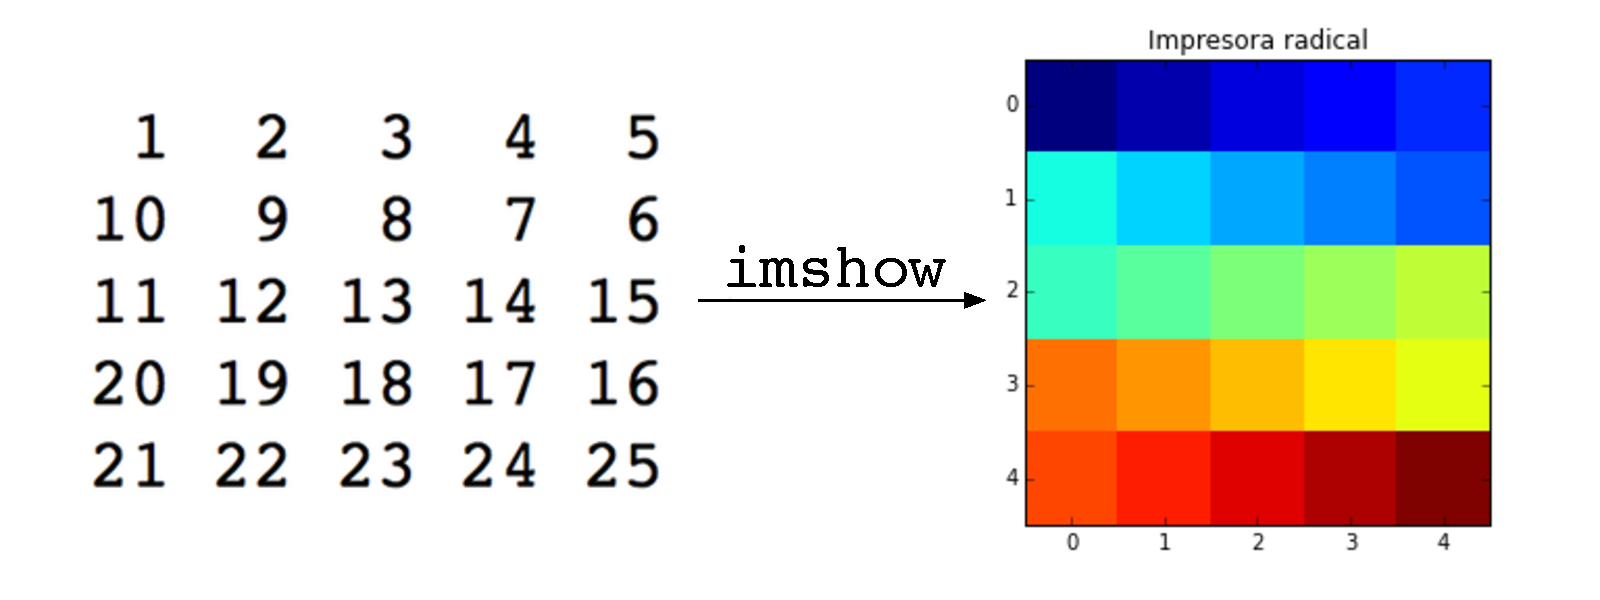
\includegraphics[width=0.7\textwidth]{./radical.pdf}
\end{center}

\end{parts}
\question[28] {\bf{Carta Celeste}} \\
El archivo \verb+visiblestars.csv+ contiene las coordenadas celestes (DEC, RA) de estrellas con magnitud visual menor o igual a $8.5$. El archivo \verb+namedstars.csv+ contiene las coordenadas y nombre de las estrellas con nombre propio. Con ellos haga un mapa celeste similar al mostrado abajo. Debe usar las siguientes rutinas:
\begin{parts}
	\part[4] \verb+genfromtxt+ para importar el archivo \verb+visiblestars.csv+,
	\part[4] \verb+genfromtxt+, con la opción \verb+dtype=None+, para importar el archivo \verb+namedstars.csv+,
	\part[4] \verb+xlim+ y \verb+ylim+,
	\part[4] \verb+xlabel+ y \verb+ylabel+,
	\part[4] \verb+plot+ para poner en un punto pequeño en la posición de cada estrella en \verb+visiblestars.csv+ y un punto rojo y más grande en la posición de cada estrella con nombre propio,
	\part[4] \verb+ms+ al usar \verb+plot+ para poner un tamaño adecuado a los puntos,
	\part[4] \verb+text+ para poner una etiqueta con el nombre de cada estrella en \verb+namedstars.csv+, y en él usar las siguientes opciones \\ \verb+fontsize=10,bbox=dict(facecolor='white',alpha=0.7),+ \\ \verb+verticalalignment='bottom',horizontalalignment='left'+.
\end{parts}


\begin{center}
	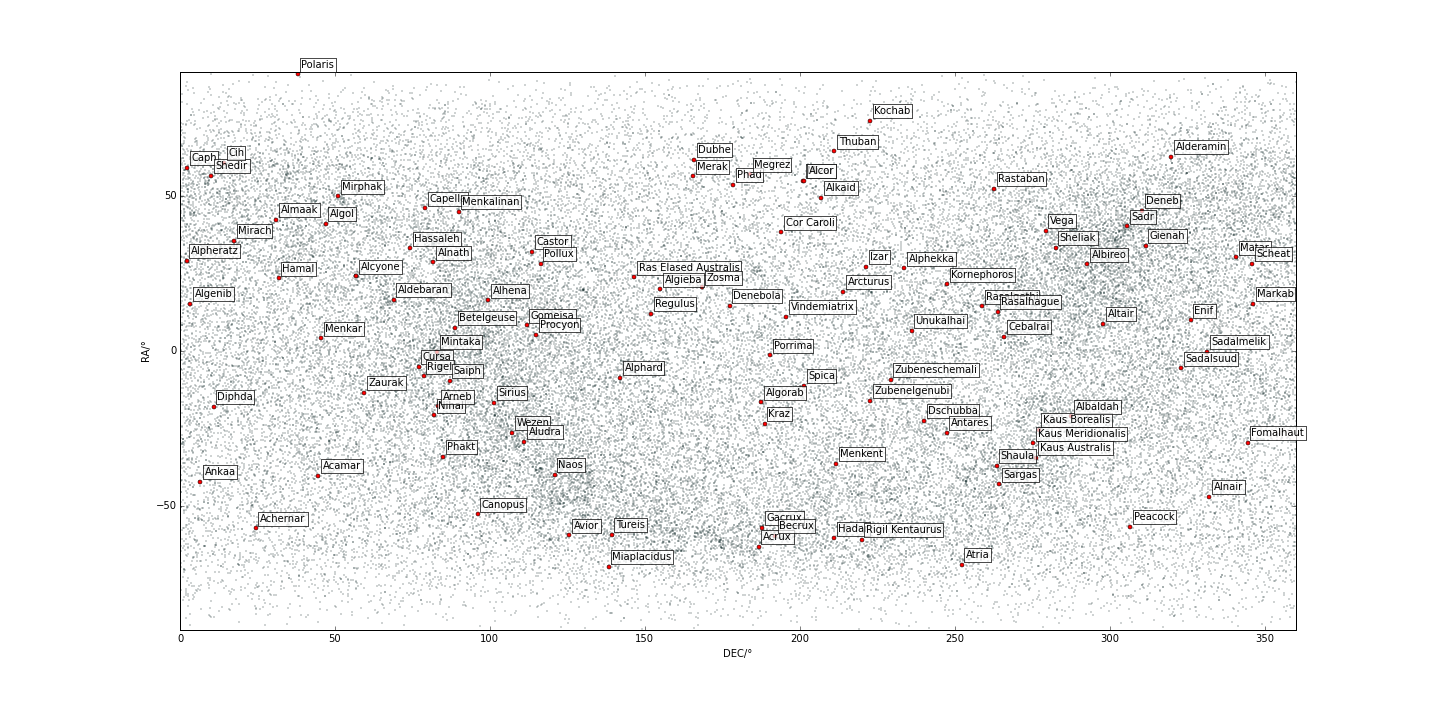
\includegraphics[width=0.95\textwidth]{./starchart.png}
\end{center}

\question[52] {\bf{Bosón de Higgs}} \href{http://www.sciencedirect.com/science/article/pii/S0370269312008581}{$\rightarrow$ el artículo}  \href{http://www.nature.com/news/higgs-triumph-opens-up-field-of-dreams-1.10970}{$\rightarrow$ la noticia} \\ 
Más abajo se muestra\footnote{CMS Collaboration, Physics Letters B. Physics Letters B 716, 30–61 (2012).} una de las gráficas que evidencia la existencia del bosón de Higgs. Sobre la gráfica se muestran los datos experimentales con barras de error y los ajustes $Ev$ y $Ev^*$. Los datos experimentales están contenidos en el archivo \verb+higgs.csv+ con las abscisas en la primera columna y las ordenadas en la segunda. $Ev$ y $Ev^*$ están dadas por las ecuaciones

\[
Ev\left(m_{\gamma\gamma}\right) = A_0 + A_1 m_{\gamma\gamma} + A_2 m_{\gamma\gamma}^2 + A_3 m_{\gamma\gamma}^3
\]
\[
\textrm{con } A_0 = 27890, A_1 = -526.3, A_2 = 3.410, A_3 = -0.007502,
\]
\[
\textrm{y } Ev^*(m_{\gamma\gamma}) = Ev\left(m_{\gamma\gamma}\right) + C e^{-\frac{(m_{\gamma\gamma}-m^*)^2}{D}}
\]
\[
\textrm{con } C = 116, m^*=125, D = 4.2.
\]

Escriba un programa en Python que reproduzca la gráfica y que haga todo lo siguiente: 
\begin{parts}
\part[5] importar el archivo \verb+higgs.csv+,
\part[5] fijar el tamaño de la gráfica para que sea cuadrada con $8$  pulgadas de lado,
\part[5] fijar el tamaño de la fuente en $15$ pt, 
\part[5] hacer la gráfica de dispersión de \verb+higgs.csv+ con barras de error verticales de $35$ unidades, 
\part[5] calcular arrays de acuerdo a las definiciones de $Ev$ y de $Ev^*$ en el intervalo de energías de $105$ a $153$ GeV,
\part[5] hacer las gráficas de $Ev$ y de $Ev^*$ con su estilo de línea correspondiente,
\part[5] poner el título usando \LaTeX  $\,$ donde sea necesario,
\part[5] rotular los ejes usando \LaTeX  $\,$ donde corresponda, 
\part[6] poner la leyenda,
\part[6] y exportar la gráfica al archivo \verb+CMSHiggs.pdf+.
\end{parts}

\begin{center}
	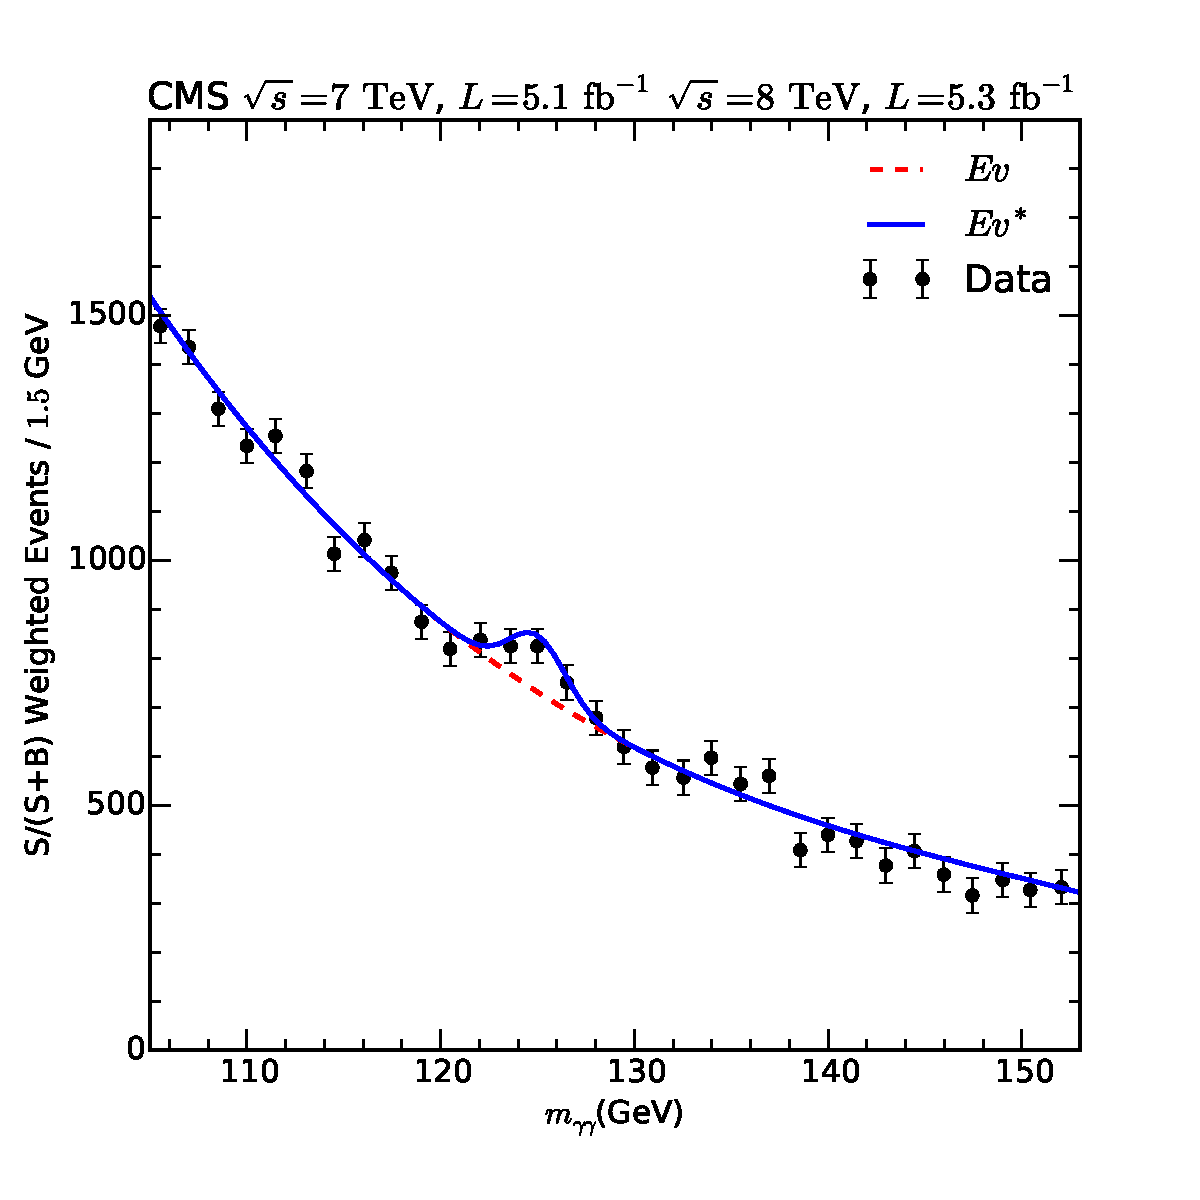
\includegraphics[width=0.9\textwidth]{./CMS-Higgs.pdf}
\end{center}

\end{questions}
\end{document}